\documentclass[twocolumn]{article}
%\documentclass{article}
%\usepackage{ctex} % 支持中文
\usepackage[utf8]{inputenc}
\usepackage{amsmath}  % 数学符号
\usepackage{amsfonts} % 黑板粗体字母
\usepackage{epstopdf}

\usepackage{algorithm}
\usepackage{algorithmic}
\usepackage{enumitem} % 使用列表
\usepackage{indentfirst}

\usepackage{caption}
\usepackage{subfigure}
\usepackage{graphicx}
\usepackage{titling} % 用于自定义标题页

% 修改页边距
\usepackage[top=1.3cm, bottom=1.3cm, left=1.2cm, right=1.2cm]{geometry}

\title{\LARGE \textbf{Network Task Management with Large Language Models}}
\author{Wang Wenbo \\ \texttt{24064411G} \and Zhou Shiyi \\ \texttt{24116285G} \and Zhang Zhihao \\ \texttt{24044588G}}
\date{\today}

\begin{document}
\captionsetup[figure]{labelfont={bf},labelformat={default},labelsep=period,name={Figure }}

\begin{titlepage}
    \centering
    \vspace*{2cm}
    {\Huge\bfseries Network Task Management with Large Language Models\par}
    \vspace{2cm}
    {\Large\itshape Wang Wenbo, Zhou Shiyi, Zhang Zhihao\par}
    \vfill
    {\large A report on NetLLM: Efficient LLM Adaptation for Network Tasks\par}
    \vspace{1cm}
    {\large \today\par}
\end{titlepage}

\maketitle
\tableofcontents
\newpage

\section{Background}
Network systems require sophisticated control algorithms to optimize performance across diverse, dynamic conditions. These management approaches have evolved through distinct methodological paradigms, each with characteristic strengths and limitations.

\subsection{Rule-based Algorithms}
Rule-based algorithms implement handcrafted heuristics to optimize network performance through explicit control rules. Examples include Copa's delay-based congestion control mechanisms and PANDA's bandwidth estimation for video bitrate adaptation. These systems have demonstrated reliable performance in production environments.

However, rule-based approaches fundamentally rely on manual engineering efforts. Network specialists must design, implement, and validate custom rules for each networking scenario. This process becomes increasingly burdensome as network environments grow more complex, limiting adaptability and scalability across diverse operational conditions.

\subsection{Learning-based Algorithms}
Deep neural networks (DNNs) trained through supervised or reinforcement learning have emerged as powerful alternatives to rule-based systems. These approaches have demonstrated superior performance across multiple networking domains including traffic classification, congestion control, and adaptive bitrate streaming.

Despite their advantages, learning-based solutions face significant challenges:

\subsubsection{High Model Engineering Cost}
Performance critically depends on specialized DNN architectures tailored to specific networking tasks. This requires substantial expertise in both networking and deep learning. Even when adapting established architectures like Transformers, engineers must manually configure attention mechanisms, tokenization schemes, and other task-specific components. This shifts the burden from rule engineering to model engineering without eliminating the fundamental design overhead.

\subsubsection{Low Generalization}
Models trained on specific network distributions frequently underperform when deployed in novel environments. For example, ABR models optimized for stable network conditions often fail under dynamic bandwidth fluctuations. This generalization gap undermines operational confidence compared to more predictable rule-based systems, limiting practical deployment despite theoretical performance advantages.

\subsection{LLM Method}
Recent advancements in large language models (LLMs) suggest potential for developing foundation models for networking tasks. These pre-trained systems with billions of parameters demonstrate emergent capabilities in planning, pattern recognition, and generalization that could benefit networking applications. However, three critical challenges must be addressed:

\subsubsection{Large Input Modality Gap}
Network monitoring produces structured numerical time-series data fundamentally different from LLMs' native text inputs. This modality mismatch prevents direct application of LLMs to networking tasks without significant input transformation and representation engineering.

\subsubsection{Inefficiency of Answer Generation}
LLMs generate outputs through sequential token prediction, which introduces:
\begin{enumerate}[itemsep=0pt, topsep=2pt, parsep=0pt]
  \item Latency unsuitable for real-time network control
  \item Potential hallucination of physically invalid configurations
  \item Computational overhead incompatible with resource-constrained network devices
\end{enumerate}

\subsubsection{High Adaptation Costs}
Bridging the domain gap between natural language and networking requires extensive fine-tuning. For decision-making tasks using reinforcement learning, this process demands prolonged environment interaction that becomes prohibitively expensive given LLMs' large parameter counts. Full-parameter fine-tuning further compounds these resource requirements.

Addressing these challenges represents a critical research direction for leveraging LLMs' capabilities in networking applications while overcoming their fundamental limitations.

\section{Innovation}

\subsection{NetLLM}

NetLLM represents the first framework specifically designed to efficiently adapt Large Language Models (LLMs) for networking applications. This innovative approach enables the use of a single LLM (such as Llama2) as a foundation model to tackle various networking tasks without requiring modifications to the base model while achieving enhanced performance. NetLLM consists of three core components:

\subsubsection{Multimodal Encoder}
The multimodal encoder functions at the input side of the LLM to effectively process diverse input information typical in networking tasks. Its primary goal is to automatically project task inputs from various modalities into the same feature space as language tokens, enabling the LLM to understand and utilize this information for problem-solving. The encoder operates through:

\begin{enumerate}[itemsep=0pt, topsep=2pt, parsep=0pt]
  \item Modality-specific feature extractors that process raw inputs from various sources relevant to networking
  \item Trainable projection layers that convert these features into token-like embedding vectors compatible with the LLM's input requirements
\end{enumerate}

This approach allows the LLM to seamlessly work with non-textual data types common in networking applications, bridging the modality gap that typically limits LLM applications in technical domains.

\subsubsection{Networking Head}
To address the inefficiency of traditional token-based answer generation, NetLLM replaces the default language modeling head with specialized networking heads at the output side of the LLM. These networking heads are lightweight trainable projectors that map the LLM's output features directly into task-specific answers.

Rather than generating tokens autoregressively, these heads enable the LLM to produce valid answers in a single inference step by directly outputting from the valid range of possible answers (e.g., selecting a bitrate from candidate options). This approach:

\begin{enumerate}[itemsep=0pt, topsep=2pt, parsep=0pt]
  \item Eliminates the risk of hallucination and invalid outputs
  \item Significantly reduces generation latency
  \item Ensures reliability for time-sensitive networking applications
\end{enumerate}

\subsubsection{DD-LRNA}
The Data-Driven Low-Rank Networking Adaptation (DD-LRNA) scheme drastically reduces fine-tuning costs while enabling the LLM to acquire domain-specific knowledge for networking. This scheme incorporates:

\begin{enumerate}[itemsep=0pt, topsep=2pt, parsep=0pt]
  \item A data-driven adaptation pipeline that works for both prediction and decision-making tasks
  \item For decision-making tasks, it employs efficient data-driven reinforcement learning techniques that eliminate time-consuming environment interactions by using an experience pool collected from existing networking algorithms
  \item Introduction of additional trainable low-rank matrices (accounting for only 0.31\% of total parameters) that efficiently capture networking knowledge
\end{enumerate}

This approach reduces GPU memory requirements by 60.9\% and training time by 15.1\% compared to full parameter fine-tuning.

\subsection{Networking Tasks}

\subsubsection{Tasks}
NetLLM is evaluated on three representative networking tasks that cover different learning paradigms and input modalities:

\begin{enumerate}[itemsep=0pt, topsep=2pt, parsep=0pt]
  \item \textbf{Adaptive Bitrate Streaming (ABR)}: A reinforcement learning model that dynamically adjusts chunk-level bitrates based on network conditions and playback buffer length during video streaming. The objective is to maximize Quality of Experience (QoE) by balancing factors like chunk bitrate, bitrate fluctuation, and rebuffering time.

  \item \textbf{Cluster Job Scheduling (CJS)}: Uses reinforcement learning to schedule incoming jobs within a distributed computing cluster. Each job is represented as a directed acyclic graph (DAG) describing execution stage dependencies and resource demands. The scheduler selects which job stage to run next and allocates computing resources to minimize average job completion time.

  \item \textbf{Viewport Prediction (VP)}: A supervised learning task that predicts a viewer's future viewport positions based on historical viewport data and potentially video content information. This is crucial for immersive video streaming systems (e.g., 360° videos) where only content within the viewer's viewport is streamed in high quality to reduce bandwidth consumption.
\end{enumerate}

\subsubsection{Why These Tasks?}
These tasks were selected for several strategic reasons:

\begin{enumerate}[itemsep=0pt, topsep=2pt, parsep=0pt]
  \item They cover both major learning paradigms commonly used in networking: supervised learning for prediction tasks (VP) and reinforcement learning for decision-making tasks (ABR and CJS).
  \item They include both centralized control (CJS, where the scheduler manages the entire cluster) and distributed control (ABR, where clients independently select bitrates) networking scenarios.
  \item They involve diverse input modalities that represent the primary data types encountered in networking tasks, including time-series data, graphs, and multimedia content.
\end{enumerate}

VP was specifically chosen as it encompasses multiple input modalities and requires cross-modality fusion, making it more challenging for LLM adaptation than prediction tasks with single input modalities (e.g., bandwidth prediction). Together, these tasks ensure that the evaluation is representative and applicable to a wide range of networking scenarios.

\subsection{Handling LLM Challenges}

\begin{figure}[t]
  \centering
  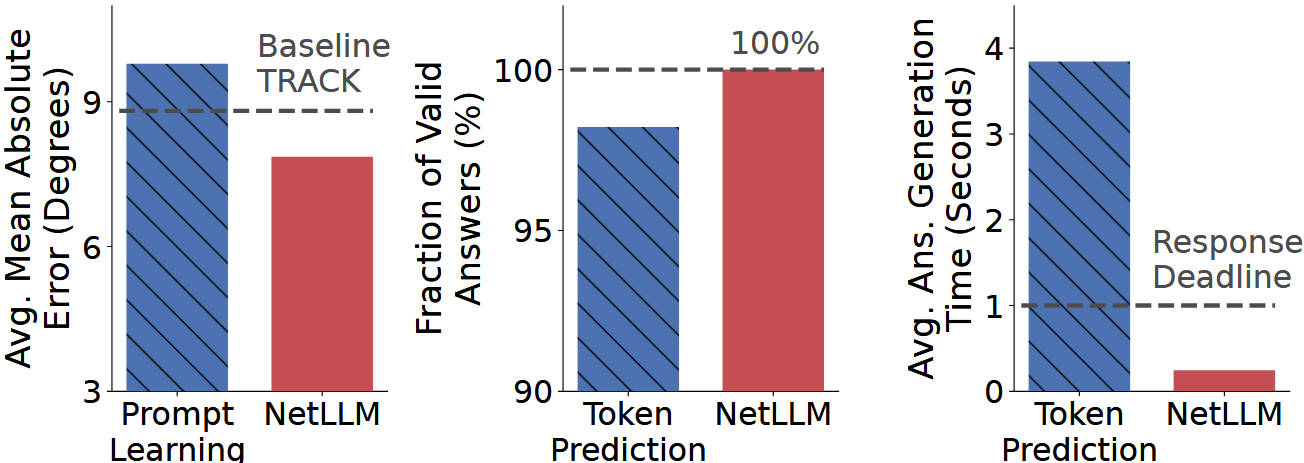
\includegraphics[width=1\linewidth]{img/figure2.jpg}
  \caption{\textbf{Illustration of the ineffectiveness for some natural alternatives with VP task as the example. Left: Prompt learning that transforms data into textual prompts achieves sub-optimal performance, while NetLLM with a multimodal encoder to encode task input data effectively outperforms baseline. Middle, Right: Token-based prediction with LM head fails to guarantee valid answers and produce stale responses, while NetLLM efficiently addresses these issues with the networking head module.}}
  \label{fig:2}
\end{figure}

\subsubsection{Large Modality Gap}
Networking tasks involve diverse input modalities (time-series data, graphs, images, etc.) that are incompatible with LLMs' text-based input format. This creates a substantial modality gap that prevents direct utilization of LLMs for networking tasks.

While prompt learning approaches that transform data into textual prompts might seem like a solution, they fall short in networking for two reasons: (1) complex modalities like images and graphs cannot be effectively transformed into text, and (2) even when transformation is possible (e.g., time-series data), the performance is suboptimal due to loss of information.

% [FIGURE PLACEHOLDER: Figure 2 (left) showing comparison between prompt learning and NetLLM performance on viewport prediction task, demonstrating NetLLM's superior performance]

NetLLM addresses this challenge through its multimodal encoder that effectively processes diverse input modalities and projects them into a feature space compatible with the LLM.

\subsubsection{Inefficiency of Token-Based Answer Generation}
The default token-based generation mechanism of LLMs presents two major limitations for networking applications:

\begin{enumerate}[itemsep=0pt, topsep=2pt, parsep=0pt]
  \item The uncertainty in token prediction increases the risk of producing physically invalid answers (hallucination), compromising reliability for critical networking systems.
  \item Due to the autoregressive nature of token generation, LLMs often require multiple inference steps to generate a single answer, resulting in high latency that fails to meet the quick responsiveness requirements of networking applications.
\end{enumerate}

% [FIGURE PLACEHOLDER: Figure 2 (middle and right) showing the fraction of valid answers and generation time comparison between token-based prediction and NetLLM's networking head approach]

NetLLM overcomes these limitations with its networking head that directly maps the LLM's output features to valid, task-specific answers in a single inference step.

\begin{figure}[t]
  \centering
  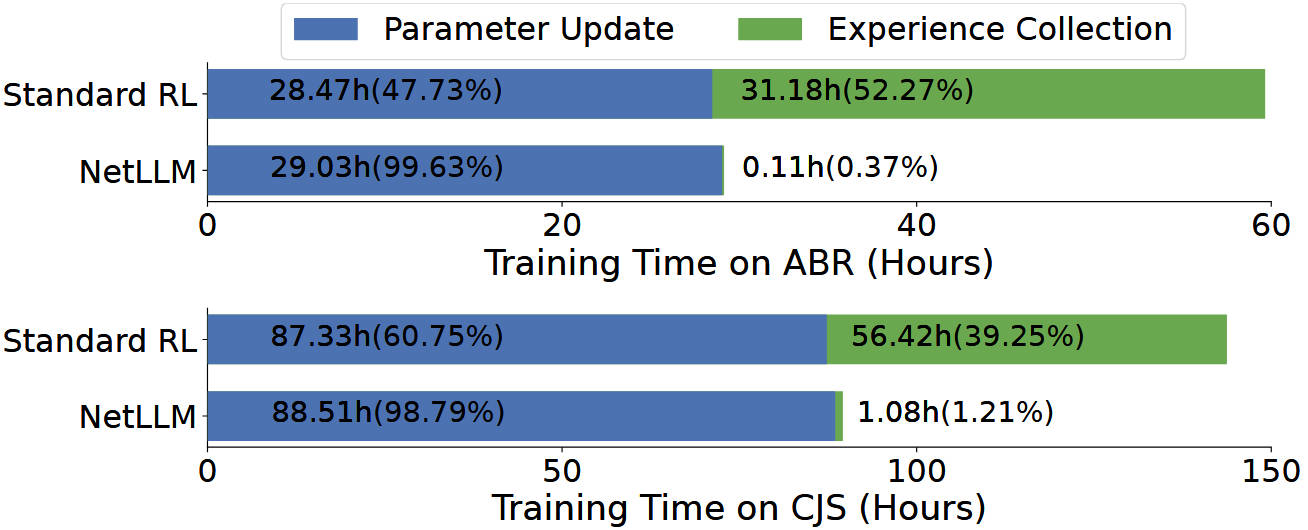
\includegraphics[width=1\linewidth]{img/figure3.jpg}
  \caption{\textbf{Using standard RL techniques to adapt LLM for RL-based decision-making tasks (ABR and CJS) incurs high training time due to the active environment interaction for experience collection. NetLLM eliminates this time-consuming process by designing an efficient data-driven adaptation pipeline in the DD-LRNA scheme.}}
  \label{fig:3}
\end{figure}

\begin{figure}[t]
  \centering
  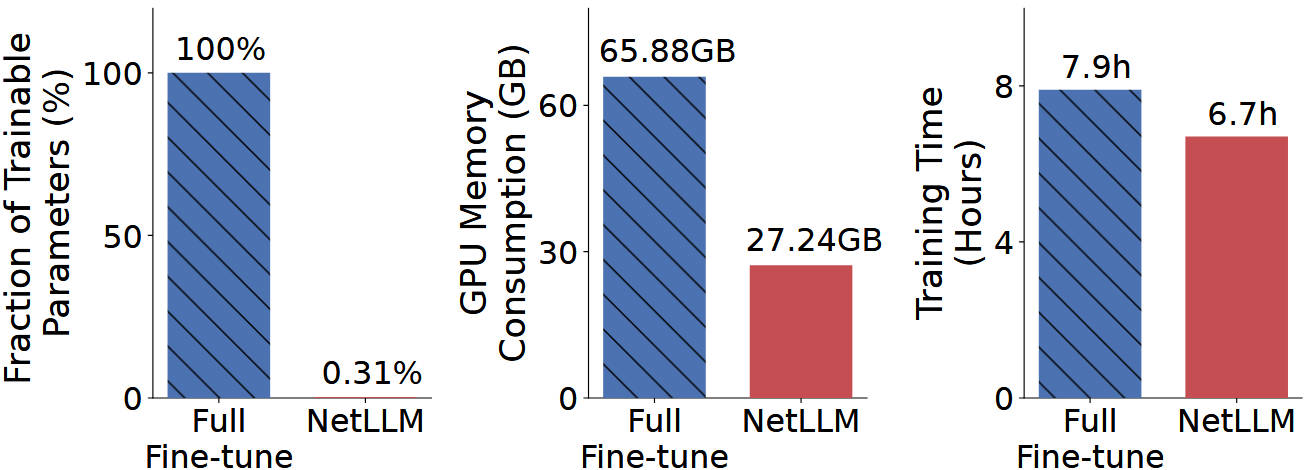
\includegraphics[width=1\linewidth]{img/figure4.jpg}
  \caption{\textbf{Illustration of the high adaptation costs of full-parameter fine-tune on the VP task. The DD-LRNA scheme of NetLLM efficiently reduces the costs by introducing a set of small trainable low-rank matrices.}}
  \label{fig:4}
\end{figure}

\subsubsection{High Adaptation Cost}
Adapting LLMs for networking tasks, particularly reinforcement learning-based ones like ABR and CJS, involves prohibitive computational costs due to:

\begin{enumerate}[itemsep=0pt, topsep=2pt, parsep=0pt]
  \item Time-consuming environment interactions required for experience collection in standard RL approaches
  \item High memory and computational requirements for fine-tuning the full parameter set of large models
\end{enumerate}

% [FIGURE PLACEHOLDER: Figure 3 showing training time comparison between standard RL and NetLLM's data-driven approach, highlighting the elimination of environment interaction time]

% [FIGURE PLACEHOLDER: Figure 4 illustrating the reduction in GPU memory and training time achieved by NetLLM's DD-LRNA scheme compared to full-parameter fine-tuning]

NetLLM's DD-LRNA scheme addresses these challenges by:
\begin{enumerate}[itemsep=0pt, topsep=2pt, parsep=0pt]
  \item Using a data-driven adaptation pipeline that eliminates the need for active environment interaction
  \item Introducing efficient low-rank matrices that capture domain knowledge while updating only 0.31\% of the model parameters
  \item Reducing GPU memory consumption by 60.9\% and training time by 15.1\%
\end{enumerate}

This approach makes LLM adaptation for networking tasks practical and efficient while maintaining high performance.

\section{NetLLM Design}

NetLLM is designed with efficient APIs and modules that can be easily integrated into existing SL and RL codebases, significantly reducing the cost of adapting LLMs to network tasks while retaining its robust pre-trained knowledge.

\subsection{API Design}
NetLLM is implemented using Python and Bash, and it uses three APIs: Adapt, Test, and RL\_Collect to interact with the existing codebase.

\begin{figure}[t]
  \centering
  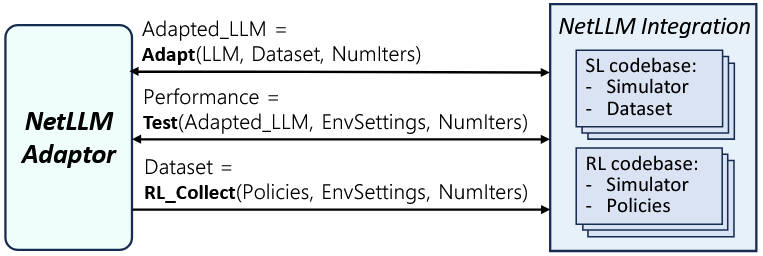
\includegraphics[width=1\linewidth]{img/figure7.jpg}
  \caption{\textbf{Components and interfaces needed to integrate NetLLM with an existing SL/RL codebase for LLM adaptation.}}
  \label{fig:9}
\end{figure}

\subsubsection{Adapt}
Use the provided dataset to adaptively tune the LLM, learn domain knowledge for a specific network task, and return an adjusted LLM snapshot.

\subsubsection{Test}
Evaluate the performance of the adapted LLM in a test environment for a given simulation setup.

\subsubsection{RL\_Collect}
For RL tasks that do not have an off-the-shelf dataset, interact with the environment using a given RL policy to collect empirical datasets for subsequent adaptation to the LLM.

\subsection{Module Implementation}
Through the design of multimodal encoders, network headers, and low-rank matrices, NetLLM can efficiently process multimodal data and generate valid answers for specific network tasks.

\begin{figure}[t]
  \centering
  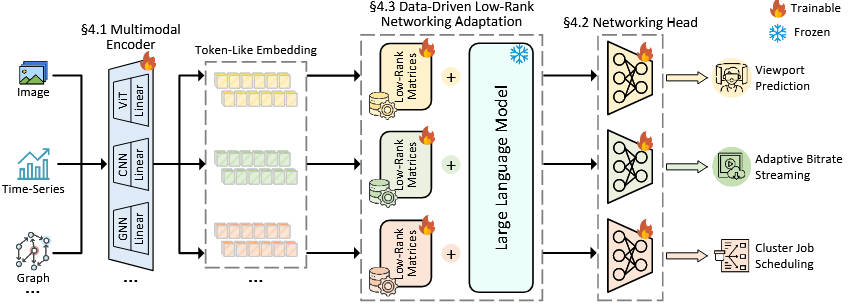
\includegraphics[width=1\linewidth]{img/figure8.jpg}
  \caption{\textbf{NetLLM consists of three core components: multimodal encoder to encode task inputs, networking head to generate task-specific answers and data-driven low-rank networking adaptation to efficiently learn domain knowledge for networking. The framework is illustrated with three tasks: VP, ABR and CJS, but all ideas can be easily applied to other networking tasks.}}
  \label{fig:7}
\end{figure}

\subsubsection{Multimodal Encoder}
The core purpose of a Multimodal encoder is to process non-textual information. Feature encoder is used to extract features using some existing high-performance feature encoders for different kinds of features. Linear projection is used to solve the problem that the extracted feature dimensions are not equal to the required input dimensions. 

The multimodal encoder encodes the multimodal input data in the network task into token-like embeddings that can be processed by the LLM. For different modalities of data, specific feature encoders are used to extract features, such as Vision Transformer (ViT) to extract image features; using 1D-CNN (One-Dimensional Convolutional Neural Network) to extract features from time series data; Extract features of scalar data using a fully connected layer and feature extracting graph data using graph neural networks (GNNs).

Finally, the extracted features are projected into the embedding space consistent with the input dimension of the LLM through a linear layer, and Layer Normalization is used to ensure the stability of the training process.

\begin{figure}[t]
  \centering
  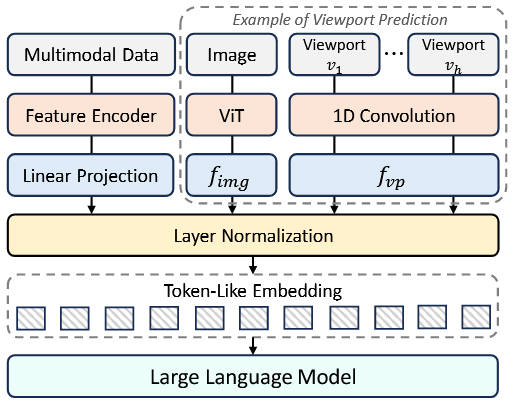
\includegraphics[width=1\linewidth]{img/figure9.jpg}
  \caption{\textbf{Illustration of the multimodal encoder of NetLLM to encode multimodal data.}}
  \label{fig:8}
\end{figure}

\subsubsection{Networking Head}
The network header designs a lightweight trainable projector for each network task, mapping the output features of the LLM directly to the task-specific answer space. Generate answers directly from the output of the LLM instead of word-by-word predictions, reducing generation delays and ensuring the validity of answers. The core role of the network header is to output non-text content.

\subsubsection{Data-Driven Low-Rank Networking Adaptation (DD-LRNA)}
DD-LRNA optimizes the model by using a static, pre-collected dataset, improving the efficiency of training and reducing the complexity and resource consumption of real-time data processing.

For prediction tasks, the LLM was fine-tuned using a standard supervised learning (SL) data-driven training process. At the same time, for decision-making tasks, data-driven reinforcement learning (RL) technology is used to fine-tune the LLM through the empirical dataset collected by the interaction between existing algorithms and the environment, so as to avoid direct interaction with the environment.

In order to retain the pre-training knowledge of LLMs, all parameters of LLMs are frozen so that they remain unchanged during the fine-tuning process, and low-rank matrices with dimensions much smaller than the original matrices are introduced, so as to significantly reduce the training cost. At each training step, a random batch of data is sampled from the dataset, fed into the LLM to generate answers, the loss is calculated, and the parameters of the low-rank matrix are updated by gradient descent.

\begin{figure}[t]
  \centering
  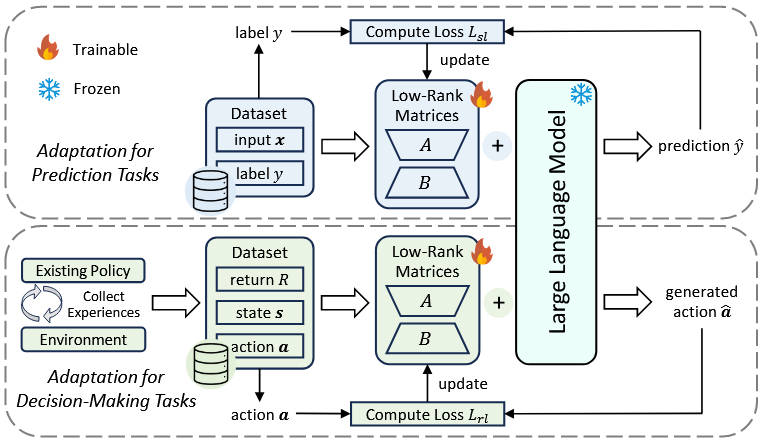
\includegraphics[width=1\linewidth]{img/figure10.jpg}
  \caption{\textbf{Illustration of the data-driven low-rank networking adaptation scheme of NetLLM.}}
  \label{fig:10}
\end{figure}

\section{Evaluation}

\subsection{Setup}
The experimental part of the paper uses Llama2-7B as the base model, adapting Llama2 via NetLLM in order to fulfil the three network tasks VP, ABR and CJS. The authors generated different simulated environments for testing to fully evaluate the performance of the model. Different baselines were used for comparison for different tasks, including learning-based algorithms (TRACK, GENET, Decima) and rule-based algorithms (e.g., linear regression, BBA, FIFO, etc.). For performance metrics, Mean Absolute Error (MAE), Quality of User Experience (QoE) scores and Job Completion Time (JCT) are used. Lower MAE, higher QoE and lower JCT indicate better performance.

\begin{figure}[t]
  \centering
  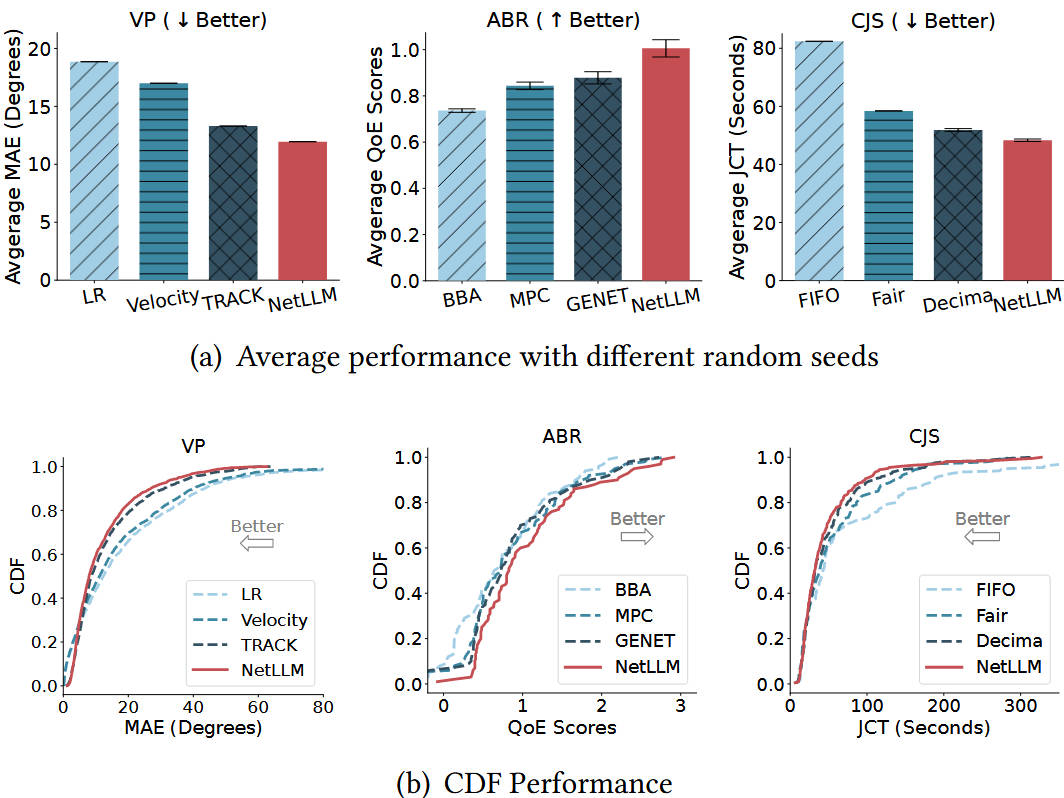
\includegraphics[width=1\linewidth]{img/figure5.jpg}
  \caption{\textbf{Comparing NetLLM-adapted Llama2 for VP, ABR, and CJS, with baselines in testing environments generated with the same settings as training environments.}}
  \label{fig:5}
\end{figure}

\subsection{General Evaluation}
The first is a general evaluation, where the NetLLM-adapted Llama2 and other methods are evaluated in a test environment with the same setup as the training environment. Figure \ref{fig:5} shows the performance comparison of the different approaches in three different tasks. It can be significantly observed that NetLLM-adapted Llama2 outperforms the other approaches in all the tasks, significantly reducing MAE, improving QoE and reducing JCT.

\begin{figure}[t]
  \centering
  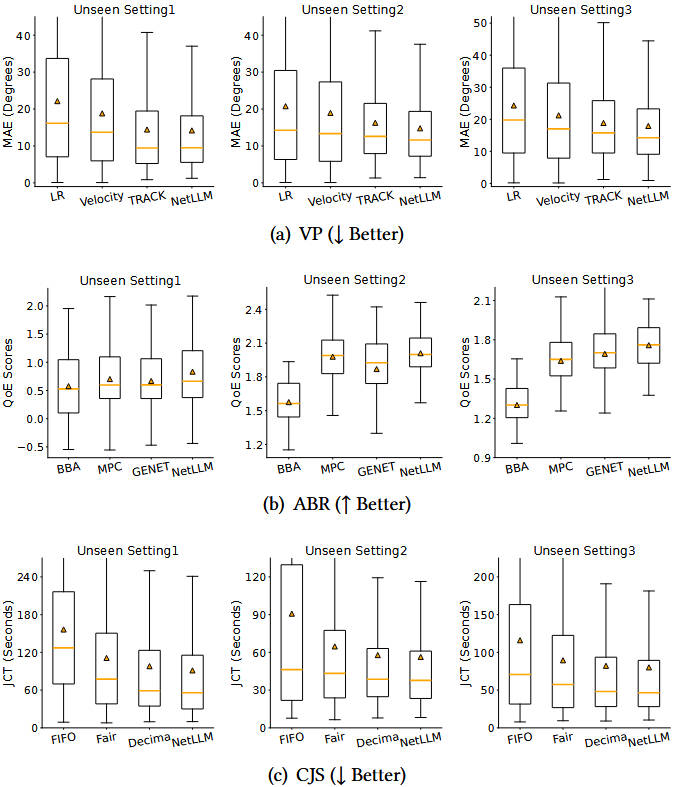
\includegraphics[width=1\linewidth]{img/figure6.jpg}
  \caption{\textbf{Comparing the generalization performance of NetLLMadapted Llama2 for VP, ABR, and CJS, with baselines in testing environments generated with settings different from training environments. The shape of box shows the distribution and the triangle in each box denotes average.}}
  \label{fig:6}
\end{figure}

\subsection{Generalization}
The paper then goes on to show a generalized evaluation of NetLLM-adapted Llama2. All methods were tested by generating environments with various settings different from the training environment. NetLLM-adapted Llama2 performed better in all test environments. Where traditional DNN models perform poorly in these unseen environments (GENET), the NetLLM framework demonstrates greater generalization. For the final experiment of the generalization ability evaluation, the authors of the paper tested and evaluated NetLLM-adapted Llama2 in a real-world client-server ABR system under different network connections. The results show that NetLLM-adapted Llama2 performs well and can be used in real-world applications.

\section{Insights And Extra Idea}

\subsection{Cons of NetLLM}
The strengths of the NetLLM framework have been explained in detail in previous sections of this report. So here we will only talk about the shortcomings of the NetLLM framework. The first is the computational overhead of the NetLLM framework. Although there are model compression techniques that can be used to try to mitigate the computational overhead, there is still a need to carefully weigh the relationship between performance and resource consumption in real-world applications. The second is that the success of the NetLLM framework in testing is somewhat dependent on the pre-trained knowledge of LLM. This can lead to limitations in specific domains or tasks in the future. The last is because the NetLLM framework does not yet have a deep enough understanding of the internal workings of the network domain, which limits its interpretability and trustworthiness in some applications.

\subsection{Extra Thoughts}
By reading this paper we appreciate the powerful generalization and migratability of LLMs. The success of the NetLLM framework represents the opening of a new field of combining LLMs with network optimization, providing new ideas and methods for wireless network intelligence. It also inspires readers to use it for exploring and trying new methods and tools when faced with complex problems.

In future research, the potential of the NetLLM framework for other network-related tasks, such as intrusion detection and network identification software, should be explored in depth. At the same time, more efficient fine-tuning methods are sought to achieve the goal of being able to further reduce computational resources and time consumption. The NetLLM framework is not only of academic interest, but may also have a profound impact on the design and optimization of physical network systems. In addition, the excellent design of NetLLM framework also has the potential of cross-domain application. For example, the multimodal encoder and network header provide new solutions to the problem of handling complex, multimodal data.

In conclusion, the NetLLM framework not only shows great potential in handling complex network tasks but also has a wide range of applications.

\section{Contributions}

\subsection{Zhang Zhihao}
Zhihao conducted an in-depth analysis of the innovations and motivations of NetLLM, wrote the background and motivation sections, and shared the findings with the team to ensure a unified understanding. He also created the corresponding slides for this part to maintain consistency in the overall presentation.

\subsection{Zhou Shiyi}
Shiyi provided a detailed analysis of the technical details of NetLLM including model architecture and algorithm design, and wrote the relevant section of the report and prepared the presentation materials. She closely collaborated with the team to ensure that the technical details accurately supported other parts of the project and was responsible for creating the slides for this section.

\subsection{Wang Wenbo}
Wenbo thoroughly interpreted the evaluation and discussion sections of the paper, summarized the effectiveness and limitations of the NetLLM method, explored potential improvements and future applications, and wrote the relevant sections of the report. She also summarized the team members' different understandings of the method and was responsible for creating the corresponding slides.

\end{document}
